\section{Background}\label{sec:background}

TODO introduction
\subsection{Spark}
Spark is the probably most widely used and industry accepted cluster computing model.
It improves over former computing models, e.g. MapReduce~\cite{mapreduce}, Hadoop or Haloop~\cite{haloop},
by allowing to cache results in memory between multiple queries, using so-called resilient distributed datasets~\cite{rdd}. % TODO sources for hadoop and haloop
However, although Spark implements most operations in memory, shuffles are an exception which still writes and reads
the whole intermediary dataset to and from disk.
Consequently, shuffling remains to be a highly expensive operation which is the bottleneck of many workflows.
Still, Spark provides the user with a general distributed data processing model with strong fault- and struggler tolerance
on commodity, shared-nothing clusters.


% TODO local mode vs cluster mode and decision to handle only local mode

% TODO tasks, executor, worker, JVM instances, master, worker
\subsubsection{Catalyst}
% TODO Catalyst chapter
Catalyst~\cite{catalyst} is Spark's query optimizer.
From a given query, e.g. an SQL query or one constructed using the DataFrame API, it constructs
in multiple stages an executable \textit{physical plan}.
\begin{figure}
    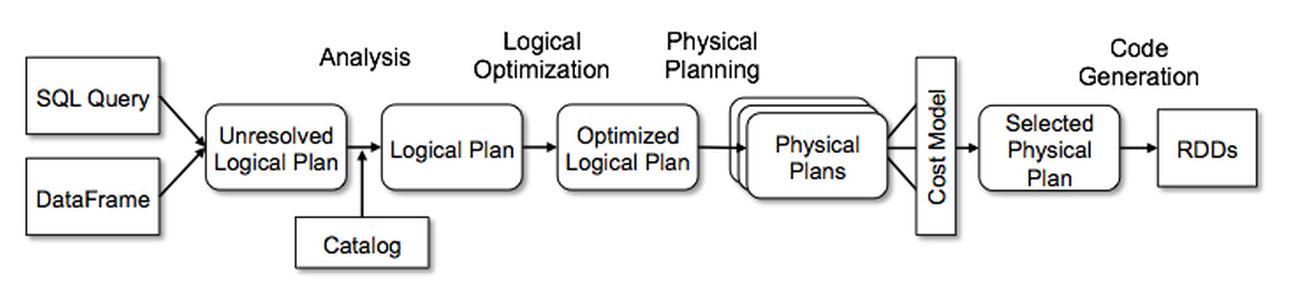
\includegraphics{figures/catalyst-stages.png}
    \caption{Input and stages of the Catalyst optimizer.}
    \label{fig:catalyst-stages}
\end{figure}
Its inputs and stages are shown in~\cref{fig:catalyst-stages}.
Below we explain these in order.

The input of Catalyst is a query in the form of a DataFrame or SQL string.
From the optimizer builds a \textit{unresolved logical plan}.
This plan can include unresolved attributes, e.g. attribute names which are not matched to a specific
data source yet or which have no known type.
To resolve this attributes Catalyst uses a \textit{Catalog} of possible bindings which describes the
available data sources.
This phase is referred to as \textit{Analysis} and results in a \textit{logical plan}.

The \texit{logical plan} represents \textit{what} should be done for the query but not exactly \textit{how},
e.g. it might contain a Join operator but not a Sort-merge join.
The logical optimization phase applies batches of rewriting rules until a fixpoint is reached.
A simple example of a logical optimization would be rewriting $2 + 2$ into $4$.

From the \textit{optimized logical plan} the optimizer generates one or multiple \textit{physical plans} by
applying so called \textit{Strategies}.
They translate a logical operator in one or multiple physical operators.
\textit{Strategies} are also allowed to return multiple physical plans for a single \textit{logical plan}.
In this case, the optimizer selects the best one according to a \textit{cost model}.

During the \textit{code generation} phase, Catalyst compiles Java byte code for some of the \textit{physical
operators}.
This code executes often magnitudes faster than interpreted versions~\cite{catalyst} of the same operator because
it can be specialized towards this particular query, e.g. if a join operates only on integers, code
generation can prune all code paths dealing with strings.
% TODO cite paper or website?
Indeed, the code generation phase is part of another Spark project called \textit{Tungsten}~\cite{tungsten}.
In this thesis, we do not build any code generated physical operators.
Hence, we do not treat this topic in depth.
It is enough to know that all freshly generated Java code is wrapped into physical operators of the type \textit{WholeStageCodeGen}
which allows seamless integration with interpreted operators.

Finally, Catalyst arrives at an optimized physical plan which implements the query.
The execution of this plan is called
\textit{structured query execution}~\cite{spark-internals-structured-query-execution}.
% TODO cite https://jaceklaskowski.gitbooks.io/mastering-spark-sql/spark-sql-QueryExecution.html
It translates the plan into RDD operations implemented by Spark cores.
Hence, the result of Catalysts query compilation is an RDD representing the query.
One should note that \textit{structured query execution} does not actually execute the query: theresult is an RDD which is a none materialized representation of the operations necessary to generate the
result.
In this thesis, we are not concerned with the internals of RDD's.
We do not need to introduce any new RDD operations or even touch Spark's core functionality.
Thanks to the extensibility of Catalyst, we can integrate worst-case optimal joins by adding one \textit{logical operator}, multiple
\texti{physical operators} and a \textit{Strategy} to translate the \texit{logical operator} in
its physical implementation.

\subsection{Worst-case optimal join algorithm}
The development of worst-case optimal joins started in 2008 with the discovery that the output size of a relational query is bound by the fractional edge number of its underlying hypergraph~\cite{agm}.
In 2012, Ngo, Porat, Re and Rudra published a join algorithm matching this bound~\cite{nprr}.
In the same year, Veldhuizen proved that the algorithm ``Leapfrog Triejoin'' used in LogicBlox, a database system developed by his company, is also worst-case optimal with regards to the
fractional edge number bound.
Both alorithms have been shown to be instances `Generic Join' in 2013 Ngo et al.~\cite{skew-strikes-back}.
Leapfrog Triejoin is the only worst-case join algorithm that has been implemented and benchmarked numerous times in widely different settings, e.g. Oxford course work, published research and a commercial database system~\cite{leapfrog,andreas,olddog,myria,ammar2018distributed,leapfrog-triejoin-schroeder}.

\subsubsection{LeapfrogTriejoin}
% TODO LFTJ chapter

\subsection{Distributed worst-case optimal join in Myria}
In 2014, a Leapfrog Triejoin variant, dubbed ``Tributary Join'', was used as a distributed join algorithm on a shared-nothing architecture called ``Myria''~\cite{myria-detailed}.
They use Tributary Join as a local, serial worst-case optimal join algorithm, combined with the Hypercube shuffle algorithm to partition the data between their machines~\cite{hypercube}.
% TODO sort out hypercube and shares usage
However, it is not obvious how well Hypercube shuffles scales because it replicates many of its input tuples~\cite{myria-detailed}.
The combination of Hypercube shuffles and Tributary Join in Myria does not scale well (speedup of 8 on 64 workers compared to the time it takes on 2 nodes) which, although unlikely to be optimal, is not investigated in great detail; we therefore, explain Hypercube shuffles in detail and show that they tend to replicate all data to all nodes for bigger graph patterns~\cref{ssec:hypercube-shuffle}.
Their approach is directly applicable to Spark.
% TODO add Graphflow paper: variable ordering studied, combination of bin + wcoj in plans, query planning first known approach, parallel
% execution?
% TODO check emptyheaded, it uses WCOJ's

\subsubsection{Shares}
% TODO rename HC Shares
We first explain how the Hypercube shuffle algorithm, \texttt{HC}, partitions data.
After, we provide an analysis of its scaling with regards to graph patterns with an increasing number of vertices.

\texttt{HC} partitions the input relationships for a multi-way join over \textit{w} worker nodes, such that, all tuples, which could be joined, end up on the same worker in a single shuffle round.
Hence, it allows running any multi-way join algorithm locally after one shuffle round.
The output of the join is the union of all local results.
\texttt{HC} realizes this partitioning by logical organizing all workers in a hypercube with one dimension per join variable; we call the number of variables \textit{A} and use $a_i$ to reference a single variable.
Each dimension has a size $p_i$, the $p_i$'s have to be chosen such that the constraint $w \ge \prod_{i}p_i$ is satisfied.  % TODO choosing problem
In other words, each worker can be addressed by its coordinate in the hypercube of the form $\{1..p_1\} \times ... \times \{1..p_A\}$.

With this topology in mind, it is straightforward to find a partitioning for all tuples from all relationships such that tuples that could join are sent to the same node.
We choose a hash function $h_i$ for each join variable which maps its values in the range of \{1..$p_i$\}.
Then each worker determines where to send the tuple it holds by hashing its join variables.
This results in a coordinate in the hypercube which is fixed for all join variables, which occur in the tuple, and unbounded for join variables not bound by the tuple.
Then the tuple is sent to all workers with a matching coordinate.
For example, assume a join with three variables $a_1$, $a_2$ and $a_3$ and tuple \textit{t} that binds $a_1$ and $a_2$ then we get the coordinates $h_{a1}(t_{a1}) \times h_{a2}(t_{a2}) \times \{0..p_{a3}\}$ and send the tuple
to all workers with a coordinate matching the first two attributes and arbitrary third component of the coordinate; the tuple is replicated across $p_{a_3}$ machines.

Next, we analyse the scalability of \texttt{HC} on growing graph patterns - that is, joins over a single relationship, the edge relationship of the graph \textit{E} and with two variables per atom.
In this context, atoms of the join can be seen as the edges of the pattern and variables as vertices.
In the following we consider the join query represented by the Datalog rule $Q(a_1, ..., a_A) = R_1(a_1, a_2), ..., R_k(a_{A-1}, a_A)$, we call $atoms(Q)$ the set of all atoms in $Q$, $p_1(R)$ and $p_2(R)$ the $p_i$ corresponding to the variables of $R$.
We use the method described in~\cite{myria-detailed} to calculate optimal shares allocation $p_1 ... p_A$.

Each worker receives $\sum_{R \in atoms(Q)} |R| / (p_1(R) * p_2(R))$ tuples under the assumption of uniform data distribution and good hash functions.
Our argument is that the tuples of each $R$ are divided onto $p_1(R) * p_2(R)$ workers - the workers that form the hypercube planes of its two variables.

In the special case of graph pattern matching where all atoms of the query are pointing to the same relationship, we can optimize \texttt{HC} shuffle such that a tuple is only sent once to a worker, although it might be assigned to it via multiple atoms.
If we apply this optimization, we can predict the probability with which each tuple is assigned to a worker using the Poisson binomial distribution.
The Poisson binomial distribution $Pr(n, k, u_0, ..., u_n)$ allows us to calculate the likelihood that $k$ out of $n$ independent, binary and differently distributed trials succeed, under the condition that the $i$'th trial succeeds with a probability of $u_i$.
We then use $n = |atoms(Q)|$, $k = 0$ and $u_i=1/(p_1(R_i) * p_2(R_i))$ to calculate the probability that a tuple is not assigned to an arbitrary, fixed worker $w$.
This allows us to predict the number of tuples assigned to each worker by $|E| * (1 - Pr(|atoms(Q)|, 0, u_0, ..., u_{|atoms(Q)|})$.

\Cref{table:workload} shows the expected percentage of tuples from $E$ assigned to each node for graph patterns of different sizes calculated using Poison binomial distribution and optimal shares assignments according to the method used in~\cite{myria-detailed}.
As we can see in this table, the number of tuples assigned to each worker grows over linear in the size of the graph pattern and that doubling the number of workers is inefficient to counter this growth.

The second observation has two reasons.
First, doubling the number of workers does not allow to double the dimensions of the hypercube - a hypercube always needs $p_1 \times ... \times p_A$ workers to be built.
Second, the number of replicated tuples increases with a growing hypercube because each tuple from $R_i$ is replicated to $\prod_{R_j \in atoms(Q)/R_i} p_1(R_j) * p_2(R_j)$; due to the fact that each tuple binds only two out of $A$ variables the tuple is replicated over many dimensions, e.g. let the bounded varibales be $a_p$ and $a_s$ then we get  $|\{0..p_0\} \times ... a_p ... \times ... a_s... \times \{0..p_A\}|$ matching worker coordinates.


%First, a hypercube of size $s$ and $A$ dimensions requires $s^A$ workers.
%Second, the replication increases with $A$ and $s$; we argue that each tuple is replicated to $(s+1)^{A-2}$ workers.
%Each tuple binds two out of $A$ variables, let's assume these are $a_p$ and $a_s$ then we have $|\{0..s\} \times ... a_p ... \times ... a_s... \times \{0..s\}|$ matching worker coordinates\footnote{The argument can be rephrased as the number of all strings of the length $A-2$ over the alphabet $\{0..s\}$}.

\begin{table}[t]
    \centering
    \begin{tabular}{lrr}
        \toprule
        Pattern  & Edges  & workload [64]/[128] \\ \midrule
        Triangle & 3                 & 0.18 / 0.12    \\
        4-clique & 6                 & 0.59 / 0.44    \\
        5-clique & 10                & 0.9  /d 0.82    \\
        House    & 5                 & 0.42 / 0.32    \\
        Diamond  & 8                 & 0.76 / 0.67    \\
        \bottomrule
    \end{tabular}
    \caption{Workload, on 64 and 128 workers, in percentage of tuples of the edge table assigned to each worker, using Poison binominial distribution to estimate the workload and the method from~\cite{myria-detailed} to determine the optimal shares configuration.}
    \label{table:workload}
    % See hc-workload-1.csv computed with a28fc458f4f8959a5af81a65f593ea22dcb8dd44
\end{table}

In light of the numbers presented in \cref{table:workload} and in line \cite{ammar2018distributed}, we conclude that the communication costs for \texttt{HC} converge towards a full broadcast for bigger graph patterns and scaling becomes increasingly inefficient.
Anyhow, \texttt{HC} is proven to be communication cost optimal for general multi-way joins in map-reduce like systems in a single round of shuffling in multiple settings~\cite{beame2013,beame2014,beame2016}.
Therefore, we decide to follow a different direction for distributing WCOJ's which we explain in~\cref{sec:goals}.


\subsection{Analysis of public real-world graph datasets}\label{subsec:graph-analysis}
TODO will include histogram of graph sizes, average outdeegree, maybe clustering coefficient and further interesting metrics, with
regards to the thesis, for (all?) graphs of the SNAP and Labaratory of Web Algorithms dataset collection.

\subsection{Compressed sparse row representation}\label{subsec:csr-background}
Compressed sparse row representation (short CSR) is a well known, low-memory representation for static graphs~\cite{csr,csr-first}.
To ease its explanation, we assume that the graph's vertices are identified by the numbers from 0 to $|V| - 1$.
However, our implementation allows the use of arbitrary vertice identifiers in $\mathcal{N}$ by storing the translation in an additional
array of size \textit{|V|}.

CSR uses two arrays to represent the edge relationship of the graph: one of size \textit{|E|} which is a projection of the edge relationship
onto the \textit{dst} attribute and a second of size \texttt{|V + 1|} which stores indices into the first array.
To find all destinations directly reachable from a source \textit{src $\in$ V}, one accesses the second array at \textit{src} for the
correct index into the first array for a list of destinations.
% TODO maybe example figure?

The CSR format has two beneficial properties in the context of this thesis.
First, it allows locating all destinations for a source vertice by one array lookup;
hence, in constant time.
Second, the representation is only, roughly, half as big than a simple columnar representation.
A uncompressed columnar representation needs $2 \times |E|$ while CSR uses only $|V| + 1 + |E|$, note that for most real-world graph |V|
<< |E| holds (see~\cref{subsec:graph-analysis}).
